\section{Research Description}
\label{sec:research}

We will describe the research in terms of our approach to addressing each
of the specific questions posed in the introduction.

\subsection{Question 1 -- What are the qualitative and quantitative benefits
that can be achieved for building daylighting and thermal management
through the use of catoptric systems?}

The benefits of natural light in human-occupied spaces are well
documented both in the research literature and in the popular
press~\cite{hhm15,Leslie03,ll01,Libby03,pce00,vandenW14},
and yet thermal effects also may be significant~\cite{bmbc13} (i.e., too much sunlight can increase temperature to unacceptable levels).
While many studies focus on the benefits of homogeneous light levels within a space~\cite{azaise13,bwkk15,gb16}, appropriate light levels may differ based on user needs.
The increased range of lighting effects offered by the independent positioning of mirrors
can provide functional benefits for people that need more or less
light, e.g., due to the age of the occupant or the task she or he is performing. For 
example, someone using a computer may want less light since the screen is a source of
artificial light while someone reading from physical media like
a book may require higher light levels. Similarly, light levels required for
vision may vary with the age of the occupants: as people get older, they tend to need 
higher light levels and increased luminous contrast. Furthermore, regardless of age,
different people tend to have have different visual acuity. Thus, developing a system 
that can provide a wide range of lighting effects using daylight rather than artificial light to accommodate these varying requirements is beneficial.

For thermal management, the literature on harvesting sunlight for
space heating is substantial (see,
e.g.,~\cite{deW75,Hunt79,kbd76,Lunde80,smf08,wo06}, and we will simply
leverage such well-understood techniques. As many sunlight-based
heating systems already use catoptric mechanisms (primarily for sun
tracking), our primary interest and contributions here will be to
integrate a sunlight harvesting system to investigate and demonstrate
dual-purpose use of catoptrics in a single cyber-physical system, both
for heating and for illumination.

In addition to investigating how (1) natural light can be redirected to achieve
different lighting effects using programmable dynamic orientation of mirrors on 
pan-tilt units, and (2) to what extent those lighting effects can achieve diverse
objectives such as energy collection, temperature control, and people's quality 
of experience in a space, we will also explore (3) how Markov decision processes 
(MDPs) can be used to generate policies automatically for multi-objective control of 
catoptric systems.  The choice of MDPs to generate such policies is motivated in part 
by the influence of stochastic factors such as wireless network packet loss between
a high-level controller and the units that control the mirrors themselves, and 
environmental effects such as cloud cover on the natural light that is available.

Another motivation for using MDPs is their efficacy in generating highly regular 
policies that can be implemented efficiently at run-time.  For example, policies for
proportional sharing of a non-preemptive resource~\cite{gtgs09,gtsg08} can be 
approximated efficiently on-line with high accuracy~\cite{gtspmgs10}.  Scenarios
that are relevant to this research, such as using multiple catoptric arrays to
provide even and consistent lighting of a collaborative work area, have similarly
regular structure that an MDP-based approach can exploit.  Our prior work also
shows that custom policies can be generated~\cite{tblwgs11,tggs10} that account for various 
nuances (e.g., in this proposed research, individual variations in visual acuity and thus 
lighting needs, as well as constraints to keep thermal effects within desired ranges).

We will start with a single objective, matching a provided image map that represents a 
desired illumination pattern, and then generalize this to include the separate goal of 
thermal energy harvesting while keeping room temperatures within a specified range.
To illustrate what we mean by an image map, Figure~\ref{fig:maps}
shows a set of arbitrary example images, associated with the mirror
positions that will create those images.  The forward problem is determining
the resulting image given the mirror positions.  The optimization problem
is determining the required mirror positions given the desired image.

\begin{figure}[ht]
\centering
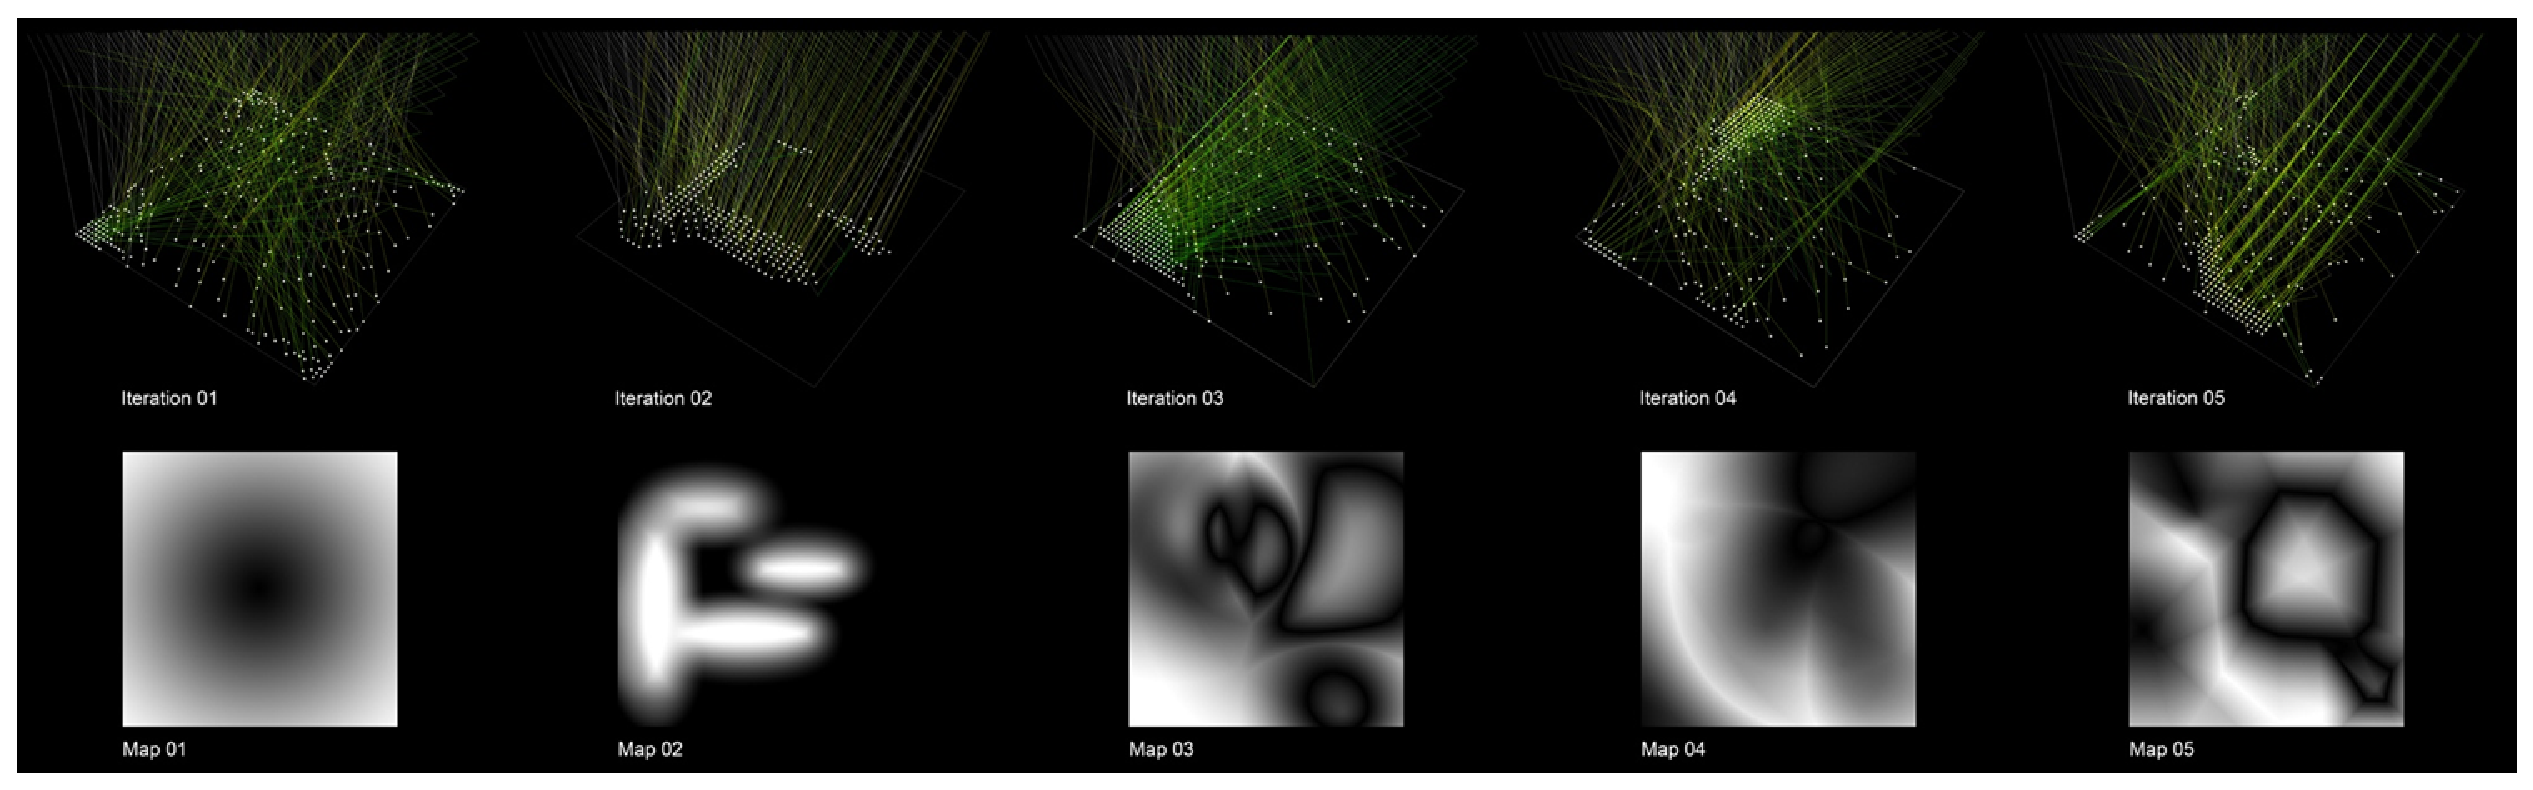
\includegraphics[width=0.9\linewidth]{figures/maps}
\caption{Example image maps (bottom) and associated mirror positioning (top).}
\label{fig:maps}
\end{figure}

For the purpose of designing an MDP, we will leverage the ability of the low-level
control mechanism to position each individual mirror as desired.  The MDP state-space 
will model higher-level management issues, e.g., which mirror should be pointed in which 
direction at which time, using distributions of mirror positioning latencies (based on 
the previous positions of the mirrors, network latency including delays due to wireless
network packet losses, etc.) and variations in natural light that we will capture through 
profiling studies.  We also will further refine these models, which intially will be based
on simply commanding the pan-tilt units to point to specific \emph{locations} in space and 
allowing the lower-level controllers to enact those commands, to a more complete cyber-physical
model in which positioning commands include specific \emph{trajectories} for each pan-tilt 
unit including its initial and final position, and the accelerations, velocities, and positions
it should adhere to in its trajectory along that path - this is important both in its
ability to enact more rapid adaptations to environmental variations and to perform dynamic
lighting effects (e.g., to get the attention of the people in a space if an emergency
alert were issued), and also in terms of tracking the wear-and-tear on the pan-tilt units and 
how that affects longevity and reliability of the catoptric arrays.

With a low-level controller in place, the state space, $\mathcal{X}$,
can encapsulate the set of mirrors pointed at each position in
the image map.  The set of actions, $\mathcal{A}$, will embody the movement
of one or more mirrors from their present position to a new position,
and the transition system, $T$, will encode the probabilistic variations
present in the available sunlight.  In the simplest case, this allows the 
reward function, $R$, to be a quantified match between the desired image 
map and the resulting daylight that is directed to each position in the physical space
(e.g., using existing image comparison quantification techniques~\cite{ds99,my09,wbo97}).
For more complex cases involving different individualized lighting requirements,
multiple objectives, etc., we will \emph{convolve} the different objective
functions to achieve a single common reward function, as we have done
in our prior work~\cite{tblwgs11,tggs10}.

After an initial exploration of the MDP formulated as described above,
we will then proceed to expand the framework to include the additional
objective of harvesting heat.  We will quantify the benefits of each
objective using general utility functions~\cite{tggs10} in a manner previously
explored by our group. One candidate set of utility functions we will
investigate will be to prioritize daylighting performance, and only
allocate excess sunlight to the HVAC subsystem. A second alternative
will be to proportionally provide sunlight to each goal up to the point
that the illumination can no longer benefit, at which point all additionally
available sunlight goes into heating.

In each of the above MDPs under investigation, we will utilize the
value-optimal solution (guaranteed to exist within Markov decision process
theory); however, this solution typically must be computed off-line, since
it is, in general, exponentially expensive to compute.  In parallel, we
will explore the space of value-optimal solutions and seek to formulate
an inexpensive to compute heuristic that closely approximates the
true value-optimal solution.

\subsection{Question 2 -- How do we provide for the safety, reliability,
maintainability, and continued efficacy of these systems?}

The ability to control mirror position is only useful over time if the
additional considerations of safety, reliability, etc., are managed
properly for the system as a whole. To address these issues, we will
investigate the degree to which they can be handled within the context
of the low-level controller versus being dealt with within the
high-level complete system control. We anticipate some of these
considerations being incorporated as constraints within the
optimization process and others as additional goals that we wish to
maximize during the multi-objective optimization itself.  Let us first
consider those that will be addressed as constraints (e.g., safety).

\paragraph{Constraints.}
A commonly used safety constraint on a positioning subsystem is to
specify hard limits on the range of motion (e.g., of each mirror, individually).
This kind of limit can be imposed by the physical design of the pan-tilt
mechanics, simply by adding physical stops at the limit positions.

The more interesting constraint systems occur when the safety considerations
are no longer locally determinable, but are dependent upon context.
An example that is relevant for our catoptric surfaces is a limit on
the total light intensity that can be supported at various positions in the
field of view of the mirrors. When providing heat into the HVAC system,
we desire a high light concentration delivered to the heat transfer point.
When illuminating a physical space for human occupants, the above
levels of light concentration are not only undesirable, they are patently
unsafe.

These context sensitive constraints add two additional requirements.
First, the higher-level management system must be responsible for them.
In our MDP formulation, we much adjust the feasible state space, $\mathcal{X}$,
so that they are unreachable (or have sufficiently negative reward as to
preclude the policy violating them~\cite{tblwgs11,tggs10}).
Second, we must also ensure that whatever choices are made by the optimization
system (whether it be via MDPs or some other approach), the actual
mirror positions are still constrained so as to not result in an
unsafe condition.  This will require feedback of some form on the actual
mirror positions and the ability to determine whether or not the actual
positions differ from the controlled positions.  This might be accomplished
either locally (e.g., via shaft encoders on the pan-tilt mechanism) or
globally (e.g., via a visual monitoring system and appropriate image analysis
software).
We will explore both options.

\paragraph{Goals.}
Many of the additional considerations are more appropriately addressed as
additional (potentially competing) goals, adding to the desires of
daylighting and heating.  An example here would be the
impact on reliability of the system when individual mirrors are moved.  As
with all electro-mechanical systems, the pan-tilt mechanism has a limited
lifetime, which can be significantly impacted by its usage duty cycle
(i.e., the more it is moved, the sooner it will fail).

This is precisely the set of circumstances in which Markov decision
processes excel. For the initial goals (of question~1), is is quite
likely that there are multiple optimal solutions (e.g., simply exchange
to pointing of two mirrors and the goals are unchanged).  However,
once we add in considerations of reliability, which is impacted by
frequency of use, we now have a much richer search space,
and a natural fit for probabilitic reward.
The MDP-based optimization approach is particularly will suited for
this type of problem, and can find optimal solutions that incorporate
minimal movement of mirrors between configurations, thereby diminishing
the maintainence costs during the normal use of the system.

The research task here is to develop, experiment with, and evaluate
Markov decision processes that simultaneously deliver daylight where it
is most beneficial, maintain the safety of the overall space,
and provide for the reliability, maintainability, and efficacy of the
catoptric surface itself.  For example, when we introduce accelerations
of the pan-tilt units into the MDP model as described above, we will bias
the reward function to avoid hard stops and rapid accelerations which both
can wear out the pan-tilt units and also may contribute to uncertainty in
positioning (similar to how wheel-slip must be addressed in mobile
robotics~\cite{mn87}).

\subsection{Question 3 -- Can we design abstractions that encapsulate
subsystems for effective reuse?}

Layered \emph{system architectures}\footnote{We use the term
\emph{system architecture}
to denote computer hardware/software architecture, distinguishing it from
architecture for the built world around us.}
have proven effective in providing standardized interfaces to
support portability
and reuse of hardware and software,
while allowing new innovations and abstractions
to enrich system capabilities.
Even when systems don't adhere strictly to standards
such as the OSI~\cite{osi} networking model or the POSIX~\cite{posix} operating
systems interface model, system designers, developers,
and users still benefit
from the structure those models provide.

This occurs largely because standardized interfaces establish clear
boundaries of responsibility on which other layers may rely, while allowing an essential
``permission to tinker'' with various implementations between those
boundaries. For cyber-physical systems, whose semantics include timing
and physical properties not considered in previous cyber-only system
architectures, there is significantly less experience with what interfaces,
abstractions, and even broad system layers are truly common (and so perhaps
could be standardized) versus which other aspects are more likely to
diverge between systems, and so should be free to do so~\cite{cag18}.
In this research, we will investigate the viability and utility of
two candidate abstractions: direct mirror control and MDP control.

\paragraph{Pan-tilt control.}
An initial version of a library (and associated programming interface) 
for pan-tilt control of our mirror units is already in place~\cite{Mitchell18}.
It is based upon an Arduino Uno microcontroller commanding the stepper
motors controlling the mirrors (up to 32 mirrors per Arduino),
with communication to the Arduino
via a USB link.  Python software executing on a Raspberry Pi coordinates
a set of up to 10~Arduinos using a USB hub.

While the initial implementation simply commands position, it is open loop
and therefore requires periodic resetting (which we accomplish by moving the
pan-tilt to the stops in each dimension), and only one motor 
connected to each Arduino can be in motion at a time.
As part of the research project, we will extend this positioning control
software in the following ways:
\begin{enumerate}

\item support closed-loop control, either through the use of shaft encoding
sensors or image-based feedback; and

\item support path direction (including acceleration profiles) in addition
to positioning commands.

\end{enumerate}

We will also extend our current prototype for mirror control to include concurrent positioning
of multiple mirrors at once -- although positioning a mirror takes only seconds currently,
the latency to adjust an entire row of mirrors in an array is noticable, and may introduce
undesirable lighting artifacts at least temporarily as mirrors are adjusted.



We also will investigate more general use of light in our approach, by adding
lenses as well as mirrors, adding color (e.g., by covering some mirrors with colored film),
and other effects. \FIXME{Chandler and Roger, please elaborate on this.}

\paragraph{MDP control.}
As is the case with pan-tilt control, we already have an initial functioning
piece of software that, given an MDP model, provides both the
value-optimal decision at any point in the design space as well as
the expected value of reward~\cite{mskgct13,tggs10}.
In the current edition, the user must provide the details of the MDP model
by authoring a set of software routines (in C++) that effectively build
an in-memory representation of the MDP model.

We will explore alternative interfaces, both textual and graphical,
for articulating the details of an MDP model.  This is particularly
challenging as the models themselves are frequently quite substantial
in size.

The MDP models themselves also will be extended to consider concurrent positioning of mirrors, in
part to ameliorate wear-and-tear on the pan-tilt units, and in part to achieve new dynamic
lighting effects that can include combinations of sequential and concurrent repositioning.

Both of these software systems (and their associated interfaces), constitute
abstractions that have strong potential for reuse in other contexts.
Pan-tilt positioning control is ubiquitious in imaging for use
with cameras (although we have a few features, such as concurrent movement
at scale, that are likely unique relative to previous systems),
and we have already used the initial versions of the MDP
software in multiple contexts~\cite{mskgct13,tggs10}.
